\subsubsection{Coloring Technique}

The \textbf{\underline{Multiplicative Schwarz method}} is inherently sequential because each subdomain's solution depends on the updated solution of the previous subdomain. \textbf{To introduce parallelism, we use a subdomain coloring mechanism}. This method \textbf{identifies independent subdomains that can be processed simultaneously by assigning different colors to different subdomains}.

\highspace
\begin{flushleft}
    \textcolor{Green3}{\faIcon{question-circle} \textbf{How does it work?}}
\end{flushleft}
\begin{itemize}
    \item[\textcolor{Red2}{\faIcon{times-circle}}] \textcolor{Red2}{\textbf{Sequential Nature of Multiplicative Schwarz}}
    \begin{itemize}
        \item[\textcolor{Red2}{\faIcon{times}}] \textcolor{Red2}{\textbf{Sequential Computation}}: The Multiplicative Schwarz preconditioner \textbf{operates sequentially}, meaning each subdomain is processed one after another.
        \item[\textcolor{Red2}{\faIcon{times}}] \textcolor{Red2}{\textbf{Limitation}}: This \textbf{serial nature limits the degree of parallelism}, \textbf{especially if there are few subdomains per color}. To overcome this, we use a coloring mechanism.
    \end{itemize}

    \item[\textcolor{Green3}{\faIcon{tools}}] \textcolor{Green3}{\textbf{Subdomain Coloring}}
    \begin{itemize}
        \item \textbf{Coloring Mechanism}: Subdomain coloring identifies independent subdomains that can be solved concurrently. \textbf{Each color represents a group of subdomains that can be processed in parallel without dependency conflicts}.
        \begin{figure}[!htp]
            \centering
            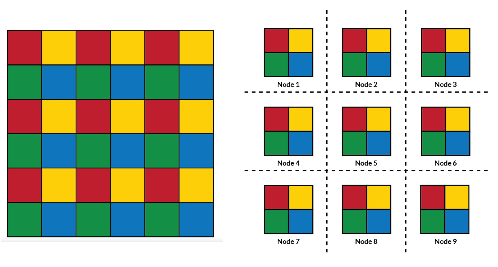
\includegraphics[width=.8\textwidth]{img/colouring-technique-1.pdf}
            \caption*{A visual representation of a grid with different colored squares (red, green, blue, yellow) and smaller grids labeled as Node 1 to Node 9. This visual aid demonstrates how subdomains are divided and colored for parallel processing.}
        \end{figure}
    \end{itemize}

    \item[\textcolor{Green3}{\faIcon{check-circle}}] \textcolor{Green3}{\textbf{Advantages and Limitations}}
    \begin{itemize}
        \item[\textcolor{Green3}{\faIcon{check}}] \textcolor{Green3}{\textbf{Degree of Parallelism}}: The \textbf{degree of parallelism depends on the number of subdomains per color}. If there are few subdomains per color, the parallelism is limited.
        \item[\textcolor{Green3}{\faIcon{check}}] \textcolor{Green3}{\textbf{Convergence Rate}}: In general, the \textbf{Multiplicative Schwarz\break method converges faster than the Additive Schwarz method}. However, the \textbf{Additive Schwarz method can achieve better parallel speedup}.
        \item[\textcolor{Green3}{\faIcon{check}}] \textcolor{Green3}{\textbf{Overall Comparison}}: The coloring technique balances the need for parallelism with the inherently sequential nature of the Multiplicative Schwarz method, ensuring faster convergence while maintaining some level of parallel computation.
    \end{itemize}
\end{itemize}
This section focuses on \textbf{enhancing parallelism in the Multiplicative\break Schwarz method by using a subdomain coloring mechanism}. This technique allows independent subdomains to be processed simultaneously, improving efficiency and convergence rates. However, the degree of parallelism is limited by the number of subdomains per color. Nevertheless, the Multiplicative Schwarz method typically converges faster than the Additive Schwarz method, although the latter may provide better parallel speedup